% !TEX root = ../Ausarbeitung.tex
\section{Einleitung}
\label{sec:Einleitung}

Bis kurz vor der Jahrtausendwende führte die Virtualisierung von Servern ein Schattendasein und jeder Service wurde auf einem dedizierten Server zur Verfügung gestellt. Dabei war es keine Seltenheit, dass Server sehr gering ausgelastet waren und der Ausfall eines nicht redundanten Servers einen Totalausfall bedeutete. Eine Beispielhafte dedizierte Serverkonstellation stellt folgende Grafik dar:
\begin{figure}[H]
	\begin{center}
		
\includegraphics[width=1\textwidth]{vm1.png}
	\end{center}
	\caption[Serverauslastung ohne Virtualisierung]{Serverauslastung ohne Virtualisierung \footnotemark}
	\label{fig:HW1}
\end{figure}
\quellefoot{1}{https://www.redhat.com/cms/managed-files/server-usage-500x131.png}
Um diese und weitere Probleme zu lösen, gewann die Virtualisierung von Servern zum Anfang des neuen Jahrtausends immer mehr an Bedeutung und ist heutzutage ein fester Bestandteil vieler großer Unternehmen. Dienste mit geringen Anforderungen werden hier auf einem System zusammengefasst:
\begin{figure}[H]
	\begin{center}
		
\includegraphics[width=1\textwidth]{vm2.png}
	\end{center}
	\caption[Serverauslastung mit Virtualisierung]{Serverauslastung mit Virtualisierung \footnotemark}
	\label{fig:HW1}
\end{figure}
\quellefoot{2}{https://www.redhat.com/cms/managed-files/server-usage-for-virtualization-500x131.png}
Doch auch die Virtualisierung von Servern birgt noch verbesserbare Nachteile. So entsteht durch das Betriebssystem der virtuellen Maschinen ein deutlicher Overhead, da diese zur Laufzeit etliche Services benötigen. Durch die virtualisierten Betriebssysteme wird die Hardware deutlich mehr beansprucht und die Startzeit ist relativ lange.
Container setzen genau an diesen Punkten an, es soll nicht für jeden Service ein zusätzliches Betriebssystem virtualisiert werden sondern der Container soll nur das zusätzlich beinhalten was er benötigt und trotzdem isoliert von den anderen Container auf der Hardware laufen.\cite{12005068320161201}\cite{redhat}
\begin{figure}[H]
	\begin{center}
		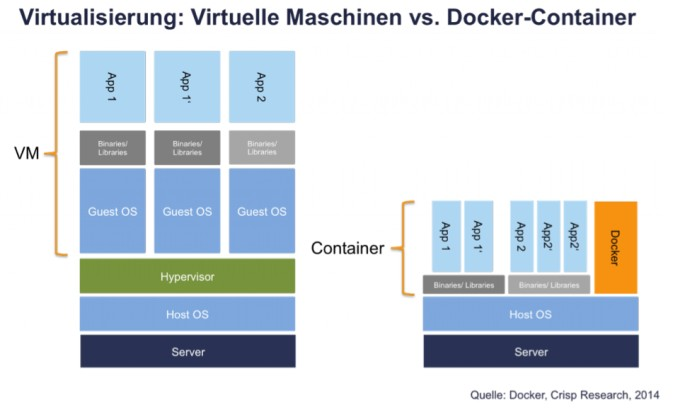
\includegraphics[width=1\textwidth]{containerundvm.jpg}
	\end{center}
	\caption[Vergleich Container und VM]{Vergleich Container und VM \footnotemark}
	\label{fig:HW1}
\end{figure}
\quellefoot{3}{https://images.computerwoche.de/bdb/2668601/738x415_f5f5f5.jpg}

